\section{Deep Embedded Clustering with Consensus Representations (DECCS)}

DECCS~\citep{Miklautz2022} addresses a fundamental limitation of existing deep clustering methods: their reliance on a single clustering algorithm whose assumptions may not match the data. Where methods like DEC~\citep{Xie2016} optimize for K-means and VaDE~\citep{Jiang2017} assumes Gaussian mixtures, DECCS instead learns a representation that simultaneously satisfies multiple heterogeneous clustering algorithms, achieving robustness through consensus. Recent surveys provide comprehensive overviews of both deep clustering methods~\citep{Min2018, Zhou2024} and consensus clustering approaches~\citep{Vega-Pons2011}.

\subsection{Consensus Clustering Background}

Traditional consensus clustering (CC) methods combine multiple clustering solutions into a single, more robust partition~\citep{Strehl2002, Fred2005}. The co-association approach of Fred and Jain~\citep{Fred2005} constructs a similarity matrix where entry $(i,j)$ counts how often instances $i$ and $j$ are co-assigned across base clusterings, then applies a final clustering to this matrix. However, classical CC methods operate on fixed representations and cannot adapt the feature space to improve consensus. Deep clustering methods like DEC~\citep{Xie2016} and IDEC~\citep{Guo2017} learn adaptive representations but are tied to single algorithms.

DECCS bridges this gap by learning a \emph{consensus representation} $Z_{cr}$ that maximizes agreement across an ensemble $\mathcal{E}$ of heterogeneous clustering algorithms. The objective function is:
\[
    f_{\Theta} = c \sum_{i=1}^{|\mathcal{E}|} \sum_{j>i}^{|\mathcal{E}|} \text{NMI}(e_i(\text{enc}_\Theta(X)), e_j(\text{enc}_\Theta(X)))
\]
where $c = \frac{2}{|\mathcal{E}|^2 - |\mathcal{E}|}$ is a normalization constant. Since NMI is not differentiable, DECCS approximates this by training classifiers to predict each algorithm's cluster assignments from the embedding, and pulling embeddings toward their consensus cluster centers.

\subsection{DECCS Methodology}

The DECCS pipeline operates in three stages. First, the encoder embeds data points into a lower-dimensional space $Z = \text{enc}_\Theta(X)$. Second, each ensemble member $e_i \in \mathcal{E}$ produces a clustering $\pi_i = e_i(Z)$ on the embedded data. Third, the encoder is updated to minimize a combined loss that includes reconstruction loss (as regularization against collapse), cross-entropy loss for predicting cluster assignments, and a consensus loss that pulls embeddings toward cluster centers weighted by inter-partition NMI agreement.

The ensemble typically includes K-means, Spectral Clustering, GMM, and Agglomerative Clustering, each capturing different aspects of cluster structure. The weighting scheme $\lambda_i = \frac{1}{|\Pi|-1} \sum_j \text{NMI}(\pi_i, \pi_j)$ downweights partitions that disagree with others, acting as an outlier filter for unreliable base clusterers.

\begin{figure}[H]
    \centering
    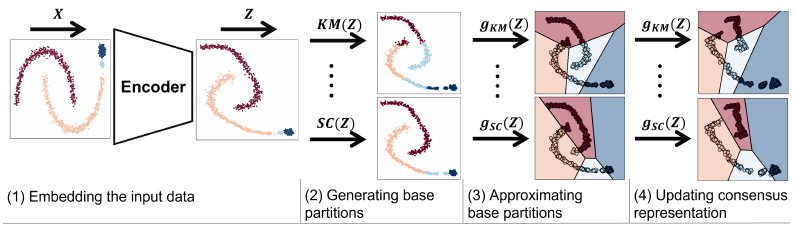
\includegraphics[width=1\textwidth]{figs/deccs.png}
    \caption{One round of the DECCS algorithm~\citep{Miklautz2022}. (1) The encoder embeds data points $X$. (2) Ensemble members $\mathcal{E}$ cluster the embeddings. (3) Classifiers predict cluster labels from $Z$. (4) The representation is updated by minimizing the combined loss $\mathcal{L}$.}
    \label{fig:deccs}
\end{figure}

\subsection{DECCS Experimental Results}

DECCS was evaluated on MNIST, Fashion-MNIST, Kuzushiji-MNIST, USPS, and other benchmark datasets using NMI and ARI as evaluation metrics. The method consistently improved agreement across all ensemble members compared to running algorithms independently, and outperformed baselines from both deep clustering and consensus clustering literatures.

\subsection{Relationship to Our Work}

Our DDECCS framework adopts DECCS's core insight---that ensembling heterogeneous clustering algorithms produces more robust results---but applies it differently. Where DECCS trains an autoencoder end-to-end with consensus loss, we apply consensus post-hoc on frozen pretrained features. This sacrifices the iterative representation refinement but gains reliability: on AwA2, K-means on frozen ResNet features (NMI = 0.872) already exceeds any result from our trained autoencoders, so the value of learned representations is limited for this dataset. Our post-hoc consensus still provides the key benefits of ensemble agreement: improved stability (near-zero variance across seeds) and better accuracy on challenging datasets like aPY (+14.4\% NMI).

\section{Deep Descriptive Clustering (DDC)}

DDC~\citep{Zhang2021} addresses a gap in the deep clustering literature: the absence of cluster-level explanations. While explainability has been extensively studied in supervised learning through methods like LIME~\citep{Ribeiro2016} and SHAP~\citep{Lundberg2017}, clustering has largely remained a black box. DDC proposes the first deep clustering framework that simultaneously learns clusters and generates concise, orthogonal descriptions for each cluster using semantic attributes.

\begin{figure}[H]
    \centering
    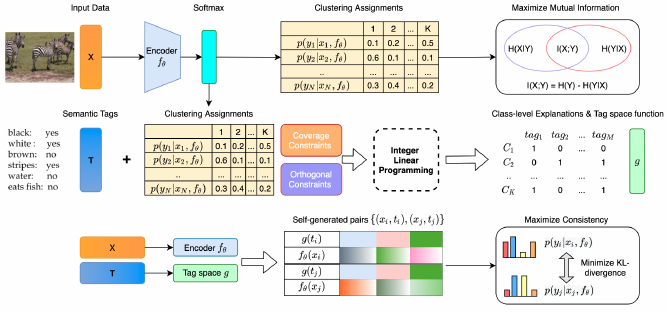
\includegraphics[width=1\textwidth]{figs/ddc.png}
    \caption{The DDC framework~\citep{Zhang2021}. Three objectives are jointly optimized: mutual information maximization for clustering, ILP-based description generation for interpretability, and self-generated pairwise constraints for consistency between the two.}
    \label{fig:ddc}
\end{figure}

\subsection{DDC Framework}

DDC's framework comprises three learning objectives. The \textbf{clustering objective} maximizes mutual information $I(X; Y)$ between inputs and cluster assignments via minimizing the loss $L_{MI} = H(Y|X) - H(Y)$, following the Regularized Information Maximization framework of Krause et al.~\citep{Krause2010}. Minimizing conditional entropy $H(Y|X)$ encourages confident cluster assignments, while maximizing marginal entropy $H(Y)$ prevents degenerate solutions where all instances collapse to one cluster.

The \textbf{explanation objective} formulates cluster description as an Integer Linear Programming (ILP) problem. Given cluster assignments and a set of $M$ semantic attributes, the ILP finds a binary allocation matrix $W$ that minimizes total tags used (conciseness) subject to coverage constraints (each cluster must have at least $\alpha$ weighted tags) and orthogonality constraints (each tag describes at most $\beta$ clusters). The ILP solution defines a mask function $g$ that filters the tag space to retain only discriminative attributes.

The \textbf{pairwise constraint loss} bridges clustering and explanation by finding instances that share similar masked tags but belong to different clusters---these represent inconsistencies that the network should correct. For each instance, the objective $J_i = \min_j \gamma |g(t_i) - g(t_j)| - |f_\theta(x_i) - f_\theta(x_j)|$ identifies partners that are close in filtered tag space but far in feature space, then minimizes KL divergence between their cluster assignment distributions. The hyperparameter $\gamma = 100$ heavily penalizes tag-space distance, ensuring that tag-similar instances are pushed together in feature space.

\subsection{DDC Architecture and Training}

DDC uses frozen ResNet-101 features fed into a 3-layer fully connected encoder network $f_\theta$ (referred to as a Multi-Layer Perceptron, or MLP, in the deep learning literature)---with dimensions [1200, 1200, K], where K is the number of clusters. The final layer applies K-way softmax for cluster assignment probabilities. Training alternates between solving the ILP (outer loop) and gradient updates on the combined loss $L = \lambda L_P + L_{MI}$ (inner loop). Tags are partially masked with probability $r$ to simulate incomplete annotation---DDC evaluates at tag ratios $r \in \{10\%, 30\%, 50\%\}$.

\subsection{DDC Results}

On Animals with Attributes (AwA, 19832 instances, 40 classes), DDC achieves NMI = 89.57 $\pm$ 1.37 at 50\% tag ratio, substantially outperforming K-means (74.23), IMG (82.16), MIC (83.43), and DAIMC (87.10). On aPY (5,274 instances, 15 classes), DDC achieves NMI = 86.30 $\pm$ 1.22, again outperforming all baselines. The ILP-generated descriptions achieve perfect Tag Coverage (TC = 1.0) on a controlled 10-class AwA subset, demonstrating strong alignment between cluster structure and semantic attributes. DDC also introduces ontology-based explanations for large numbers of clusters, where clusters sharing at least $q$ descriptive tags are connected in a graph, revealing higher-level category structure.

\subsection{Relationship to Our Work}

Our work adopts DDC's ILP formulation for cluster description generation, implementing the same conciseness objective (Eq.~2), coverage constraints (Eq.~3), and orthogonality constraints (Eq.~4). We extend the formulation with an adaptive $\alpha$ parameter that scales with attribute density, enabling the ILP to solve on sparse binary attributes (aPY, density 0.087) where DDC's fixed $\alpha = 8$ is infeasible. However, we do not implement DDC's iterative training loop with pairwise constraints---our ILP operates post-hoc on fixed cluster assignments. This means our descriptions explain the clustering but cannot improve it through the feedback loop that makes DDC's joint optimization powerful.

\section{Broader Related Work}

\subsection{Deep Embedded Clustering (DEC)}

Deep Embedded Clustering~\citep{Xie2016} pioneered the joint optimization of representation learning and clustering. DEC first pretrains a stacked autoencoder, then discards the decoder and fine-tunes the encoder using a clustering loss that minimizes KL divergence between soft cluster assignments and an auxiliary target distribution. This iterative refinement process improves both the representation and the cluster assignments. IDEC~\citep{Guo2017} subsequently showed that retaining the decoder during fine-tuning preserves local structure and prevents the embedding space from distorting catastrophically.

\begin{figure}[H]
    \centering
    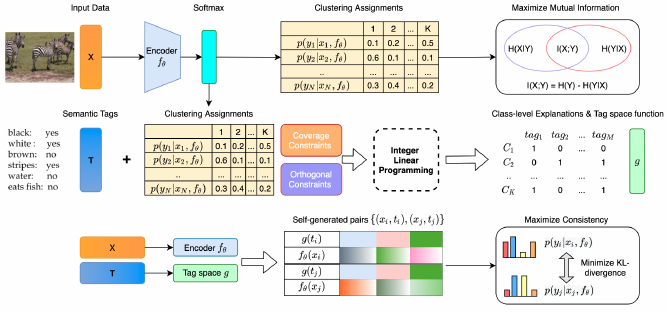
\includegraphics[width=1\textwidth]{figs/dec.png}
    \caption{Architecture of DEC~\citep{Xie2016}. A stacked autoencoder is pretrained for reconstruction, then the decoder is discarded and the encoder is fine-tuned with a clustering objective.}
    \label{fig:dec}
\end{figure}

DEC's insight---that clustering objectives can directly shape learned representations---is foundational to both DECCS and DDC. Our work builds on this lineage but takes a different approach: rather than fine-tuning representations, we use frozen pretrained features and focus on post-hoc consensus and description.

\subsection{Variational Autoencoders for Clustering}

Variational Autoencoders (VAEs)~\citep{Kingma2014} learn probabilistic mappings to latent spaces, creating smooth, continuous representations where similar data points cluster naturally. VaDE~\citep{Jiang2017} combines VAEs with Gaussian mixture models, jointly learning the latent space and cluster structure. The probabilistic framework provides principled uncertainty quantification but assumes specific prior distributions that may not match the data. VAE-based approaches create useful representations but, like DEC, lack interpretability mechanisms---they produce clusters without explaining why instances are grouped together.

\begin{figure}[H]
    \centering
    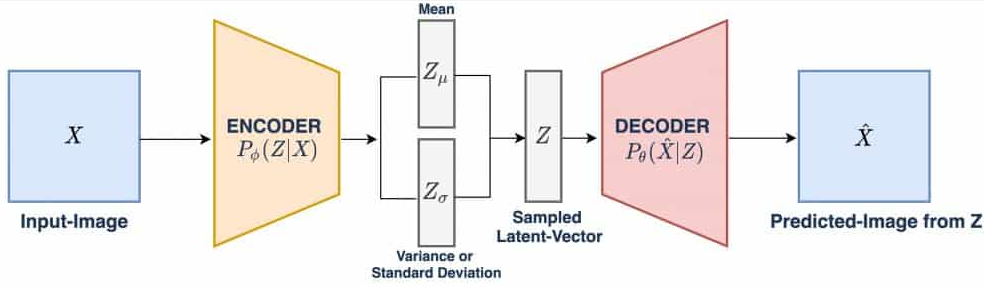
\includegraphics[width=0.8\textwidth]{figs/vae.png}
    \caption{Architecture of the Variational Autoencoder~\citep{Kingma2014}. The encoder maps inputs to parameters of a latent distribution; the decoder reconstructs inputs from samples of this distribution.}
    \label{fig:vae}
\end{figure}

\subsection{Explainable Clustering}

Explainable clustering methods fall into two categories. Explainable-by-design algorithms~\citep{Bertsimas2020, Moshkovitz2020} use interpretable features (e.g., decision trees) to simultaneously cluster and explain, but require that the clustering features themselves be human-interpretable---a condition not met by complex data like images. Post-processing explanation methods~\citep{davidson2018, Sambaturu2020} generate explanations for existing clusterings using additional semantic features, but cannot use the explanations to improve the clustering. DDC bridges both approaches by jointly optimizing clustering and explanation, while our work applies the explanation component post-hoc but benefits from consensus-based clustering quality.

Instance-level methods like LIME~\citep{Ribeiro2016} explain individual predictions through local surrogate models but do not provide the cluster-level descriptions needed in unsupervised settings. Our ILP-based descriptions operate at the cluster level, characterizing entire groups rather than individual instances.

\subsection{Contrastive Learning and Modern Deep Clustering}

Recent advances in self-supervised learning have influenced deep clustering significantly. SimCLR~\citep{Chen2020} and MoCo~\citep{He2020} learn visual representations through contrastive objectives that maximize agreement between augmented views of the same image. SwAV~\citep{Caron2020} combines contrastive learning with online clustering, contrasting cluster assignments rather than individual features. BYOL~\citep{Grill2020} demonstrates that contrastive learning works without negative pairs. These methods produce representations where simple K-means already achieves strong clustering performance~\citep{Caron2020}, supporting our finding that pretrained features can be sufficient for clustering without end-to-end training. A comprehensive survey is provided by Jaiswal et al.~\citep{Jaiswal2021}.

Contrastive clustering methods like CC~\citep{Li2021} perform instance-level and cluster-level contrastive learning jointly, while graph contrastive approaches~\citep{Zhong2021} extend these ideas to graph-structured data. Twin contrastive clustering~\citep{Shen2021} uses dual contrastive heads. These methods achieve state-of-the-art clustering performance but, like their predecessors, provide no mechanism for generating human-readable cluster explanations.

\subsection{Interpretable Consensus Clustering}

The most closely related prior work to our approach is by Gan and Allen~\citep{Gan2022}, who propose IMPACC (Interpretable MiniPatch Adaptive Consensus Clustering) in their paper ``Fast and interpretable consensus clustering via minipatch learning.'' IMPACC addresses both computational efficiency and interpretability in consensus clustering by ensembling co-occurrences from tiny subsets of observations and features (``minipatches''), using adaptive sampling to learn which features are most important for differentiating clusters. However, IMPACC's interpretability is at the \emph{feature importance} level---it identifies which input dimensions matter for clustering---rather than generating \emph{semantic descriptions} of what each cluster represents. Our approach differs in a key respect: we use DDC's ILP to produce human-readable attribute-based descriptions (e.g., ``Wheel, Pedal, Handlebars, Metal'' for a bicycle cluster), which is a fundamentally different kind of interpretability than feature importance scores. Additionally, IMPACC operates on tabular data in bioinformatics, while our DDECCS pipeline targets image datasets with semantic attribute annotations.

A recent survey on interpretable clustering~\citep{InterpClustering2024} categorizes methods into explainable-by-design, post-hoc explanation, and hybrid approaches. Our work falls in the hybrid category: the clustering itself is standard (K-means or DECCS consensus), but the ILP description module provides post-hoc semantic explanations that leverage external attribute annotations.

\section{Comparative Analysis}

\subsection{Taxonomy of Deep Clustering Methods}

Deep clustering methods can be categorized along several dimensions. Table~\ref{tab:taxonomy} organizes the main approaches by their clustering objective, supervision requirements, interpretability, and ensemble strategy.

\begin{table}[H]
    \centering
    \caption{Taxonomy of deep clustering approaches. Our DDECCS framework uniquely combines consensus clustering with semantic interpretability.}
    \label{tab:taxonomy}
    \small
    \begin{tabular}{p{3cm}p{3cm}p{3cm}p{3cm}}
        \hline
        \textbf{Dimension} & \textbf{Category} & \textbf{Examples} & \textbf{Key Feature} \\
        \hline
        \multirow{3}{3cm}{Clustering Objective}
        & Reconstruction & AE, VAE & Minimize reconstruction error \\
        & Assignment & DEC, DCN & Optimize cluster assignments \\
        & Mutual Information & DDC, IIC & Maximize MI between views \\
        \hline
        \multirow{2}{3cm}{Supervision}
        & Fully Unsupervised & DEC, DECCS & No label information \\
        & Semi-Supervised & DDC, DDECCS & Semantic attributes \\
        \hline
        \multirow{2}{3cm}{Interpretability}
        & Black-box & DEC, VAE & No explanations \\
        & Explainable & DDC, DDECCS & Generate descriptions \\
        \hline
        \multirow{2}{3cm}{Ensemble Strategy}
        & Single Algorithm & DEC, DDC & One clustering method \\
        & Consensus & DECCS, DDECCS & Multiple algorithms \\
        \hline
    \end{tabular}
\end{table}

\subsection{Feature Comparison}

Table~\ref{tab:qualitative_comparison} provides a direct feature comparison across the methods most relevant to our work.

\begin{table}[H]
    \centering
    \caption{Feature comparison of deep clustering methods. DDECCS is the only method combining ensemble clustering with interpretable descriptions.}
    \label{tab:qualitative_comparison}
    \begin{tabular}{lccccc}
        \hline
        \textbf{Feature} & \textbf{DEC} & \textbf{VAE} & \textbf{DECCS} & \textbf{DDC} & \textbf{DDECCS} \\
        \hline
        Ensemble Clustering & \xmark & \xmark & \cmark & \xmark & \cmark \\
        Semantic Supervision & \xmark & \xmark & \xmark & \cmark & \cmark \\
        Cluster Explanations & \xmark & \xmark & \xmark & \cmark & \cmark \\
        Consensus Mechanism & \xmark & \xmark & \cmark & \xmark & \cmark \\
        End-to-End Training & \cmark & \cmark & \cmark & \cmark & \xmark \\
        Pretrained Features & \xmark & \xmark & \xmark & \cmark & \cmark \\
        \hline
    \end{tabular}
\end{table}

\subsection{Computational Complexity}

Table~\ref{tab:complexity} compares the computational complexity of each method. Our pipeline's cost is dominated by feature extraction ($O(ND)$ through ResNet) and DECCS ensemble clustering ($O(mNKd)$), with the ILP contributing negligibly ($O(T^3)$ for $T = 85$ attributes). Since feature extraction is cached, repeated experiments incur only the clustering and ILP cost.

\begin{table}[H]
    \centering
    \caption{Computational complexity comparison. $N$ = samples, $K$ = clusters, $d$ = feature dimension, $m$ = ensemble size, $T$ = number of attributes.}
    \label{tab:complexity}
    \begin{tabular}{lccc}
        \hline
        \textbf{Method} & \textbf{Feature Learning} & \textbf{Clustering} & \textbf{Explanation} \\
        \hline
        DEC & $O(Nd^2)$ per epoch & $O(NKd)$ & --- \\
        DECCS & $O(Nd^2)$ per epoch & $O(mNKd)$ & --- \\
        DDC & $O(NKd)$ per epoch & $O(NKd)$ & $O(KMT)$ \\
        DDECCS & $O(ND)$ once (cached) & $O(mNKd)$ & $O(KMT)$ \\
        \hline
    \end{tabular}
\end{table}

\section{Summary and Research Gap}

This review identifies a clear gap in the literature: no existing method combines consensus-based clustering robustness with semantic interpretability. DECCS achieves robust clustering through ensemble agreement but provides no explanations. DDC generates meaningful cluster descriptions but relies on a single clustering algorithm. Our DDECCS framework addresses this gap by applying DDC's ILP-based description generation to DECCS's consensus clustering output, with the practical adaptation of frozen pretrained features replacing end-to-end training. The following chapter presents the methodology for this integration.